\section{Experimental procedure}

    The followoing task had to be done:\\
    \textbf{\ref{task_1}}: Preparation of a radio frequency resonant circuit with the insertion of an iron powde probe in a cryostate\\
    \textbf{\ref{task_2}}: Find the nuclear spin resonance by varying the NMR-pulse frequency while recording a spectrum of the $^{57}$Fe nuclear spin ensemble and calculation of the local magnetic field\\
    \textbf{\ref{task_3}}: Optimization of the pulse sequence by recording a rotation angle curve\\
    \textbf{\ref{task_4}}: Find the spin-spin- and spin-lattice relaxation constants $T_2 \text{and} T_1$.   

	\subsection{Preparation of a high frequency resonant circuit}
    \label{task_1}
    First one has to prepare a copper coil with a diameter big enough to hold an iron powder assay. After the coil is wrapped one has to sold it onto the contacts of a stick, which provides a mechanism to tune the measured frequency to find the resonance frequency. While solding one has to be careful to make sure, that one do not take to much tin, because the resisteaces of tin and copper are different. In the same way the soldered point should connect the contact and the coil directly, otherwise this could influence the results while tuning to the resonance frequency.
    \begin{center}
           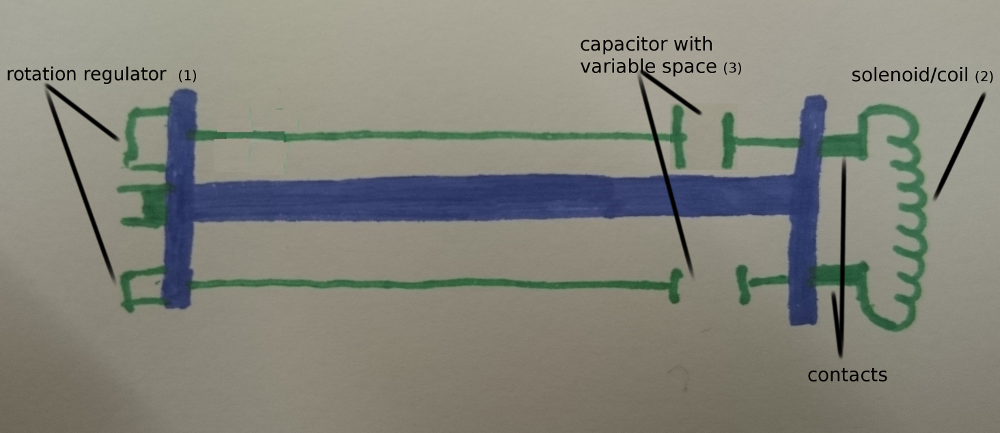
\includegraphics[scale=0.4]{pic/Skizze_Sonde.png} 
           \captionof{figure}{basic sketch of a probe with a coil on it}
           \label{fig:sketch}
    \end{center}
    The rotation regulator (\ref{fig:sketch}.1) varies the space between the capacitor's plates (\ref{fig:sketch}.3) so one can tune the frequency of the solenoid (\ref{fig:sketch}.2).
    \subsection{Finding of the nuclear spin resonance by varying the pulse frequency}
    \label{task_2}
    
    After the preparation of the solenoid and the insertion of the probe into the cryostat one has to mention what the different paramters, the measurement software has do with the curve. The different parameters one could vary are $pw$, $\tau$, $rd$ and $ad$. 
        \begin{figure}[h]
            \subfigure[intensity below resonance frequency in time domain\label{beltd}]{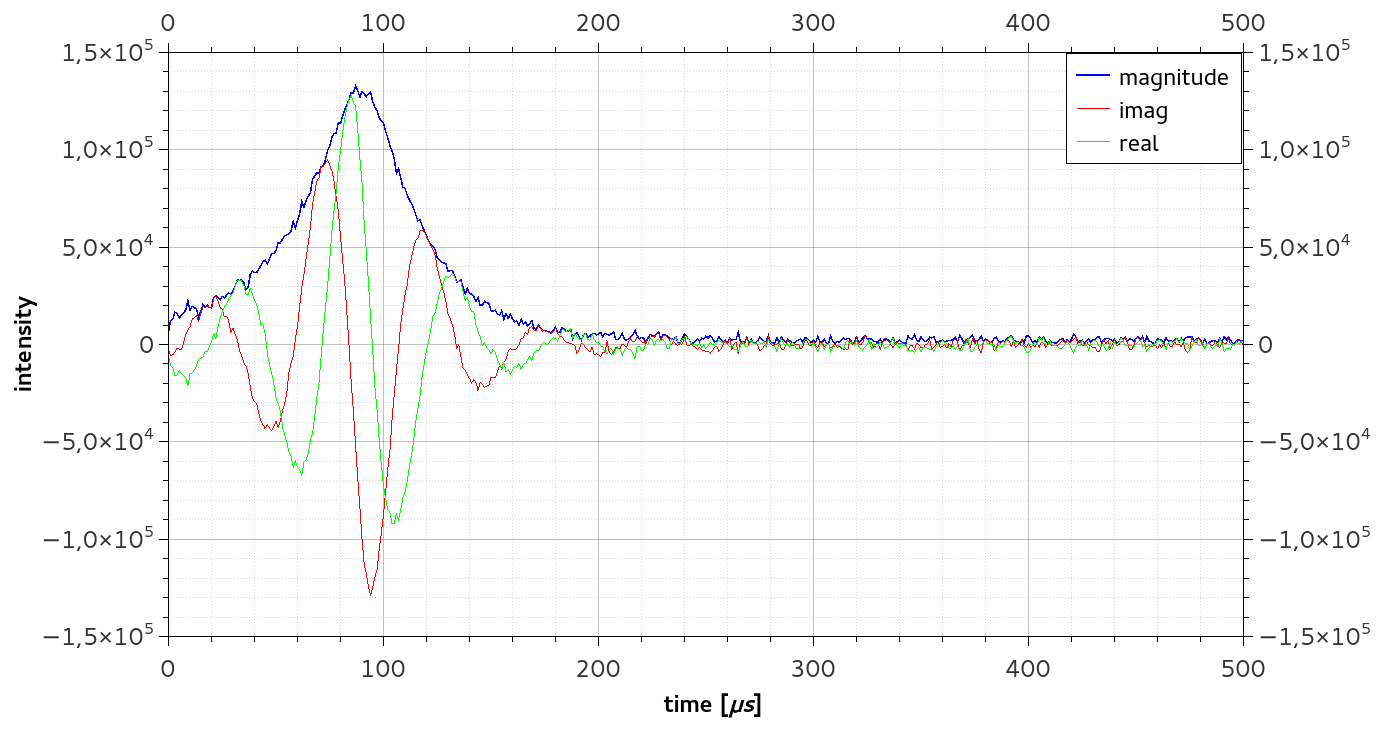
\includegraphics[scale=0.225]{pic/below_resfreq_td.png}}
            \subfigure[intensity below resonance frequency in fourier space\label{belfs}]{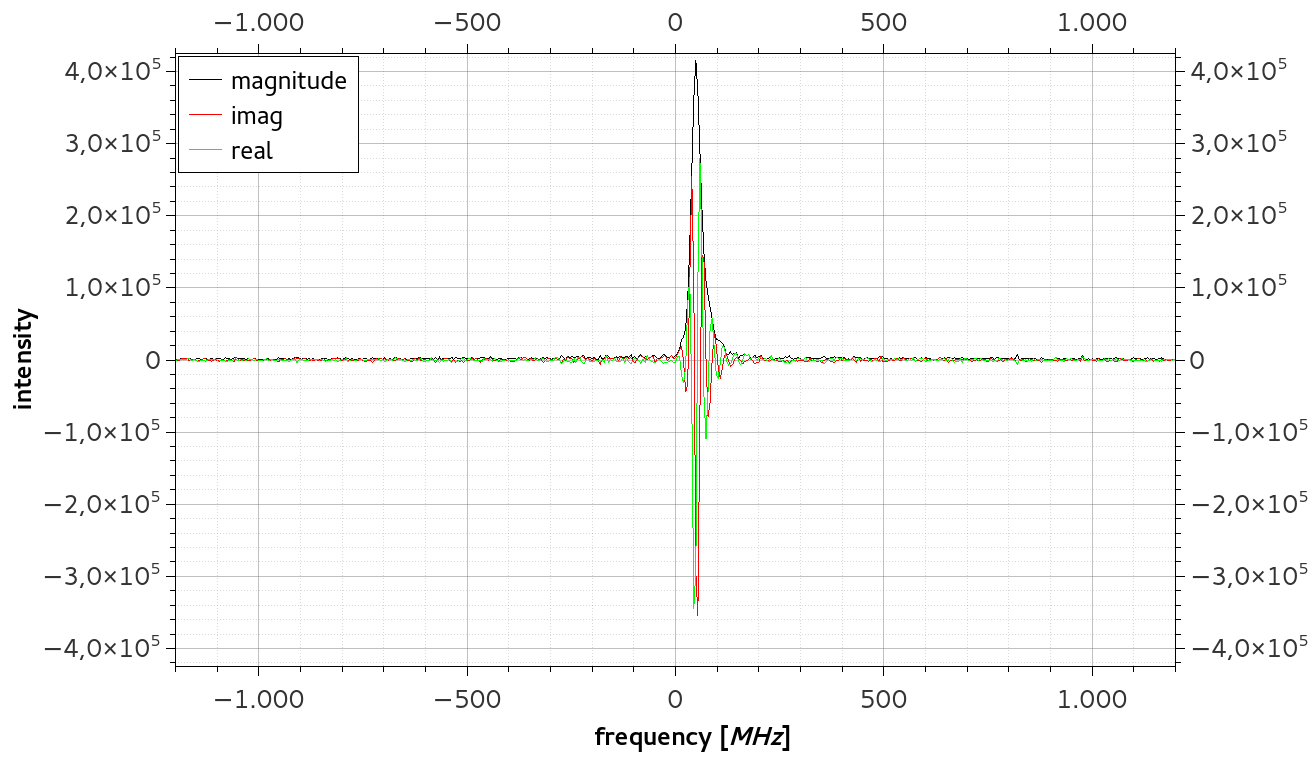
\includegraphics[scale=0.225]{pic/below_resfreq_fs.png}}
            \subfigure[intensity at resonance frequency in time domain\label{restd}]{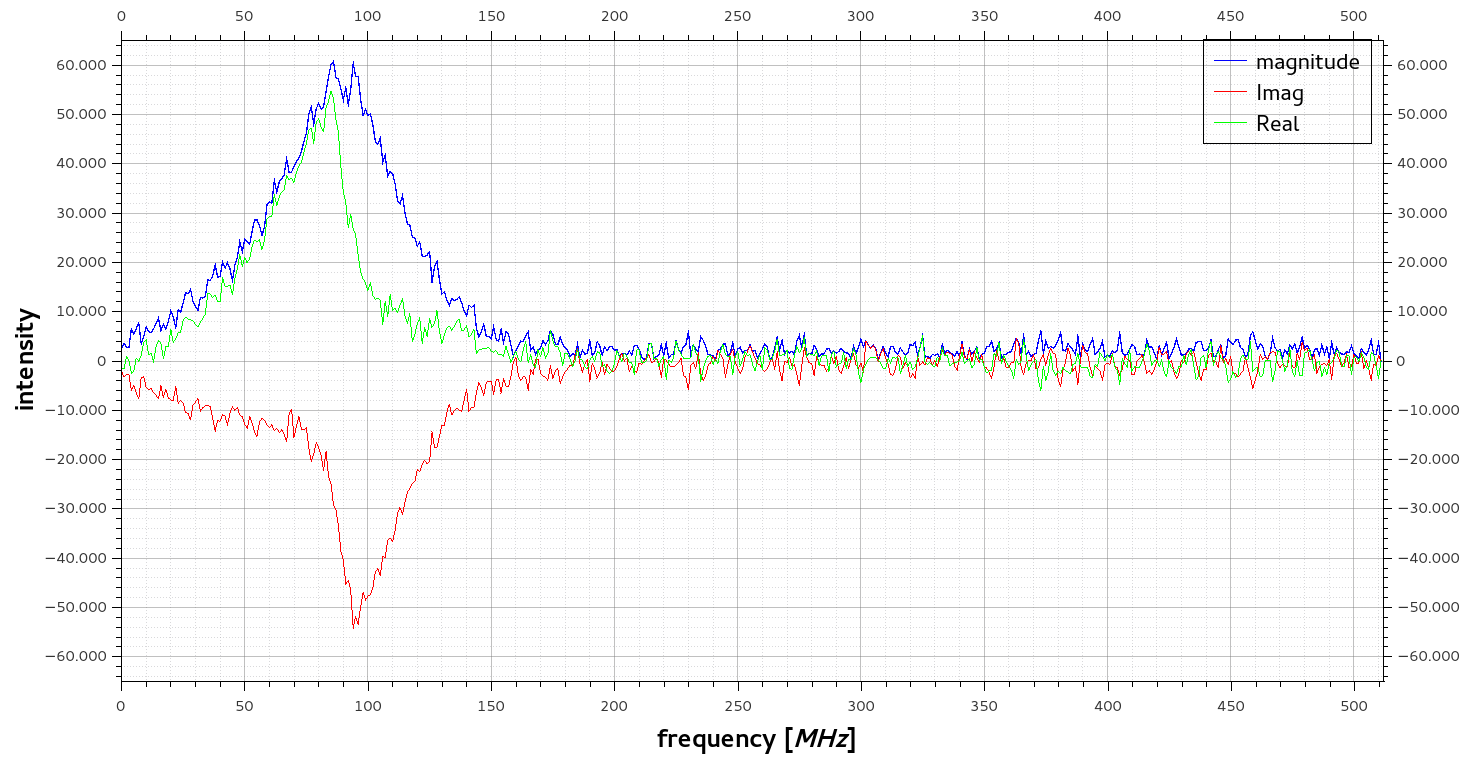
\includegraphics[scale=0.21]{pic/resfreq_td.png}}
            \subfigure[intensity at resonance frequency in fourier space\label{resfs}]{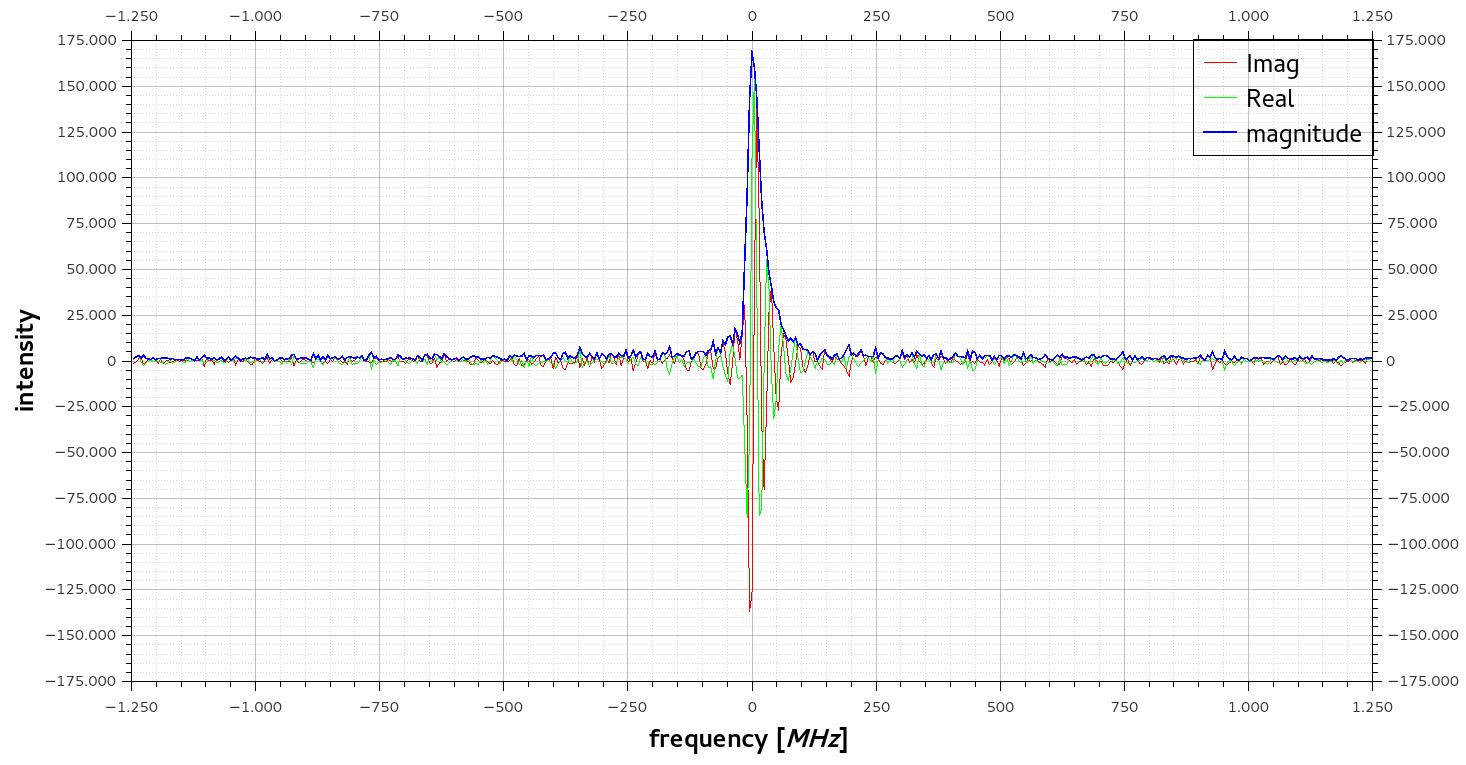
\includegraphics[scale=0.21]{pic/resfreq_fd.png}}
            \subfigure[intensity below resonance frequency in time domain\label{abotd}]{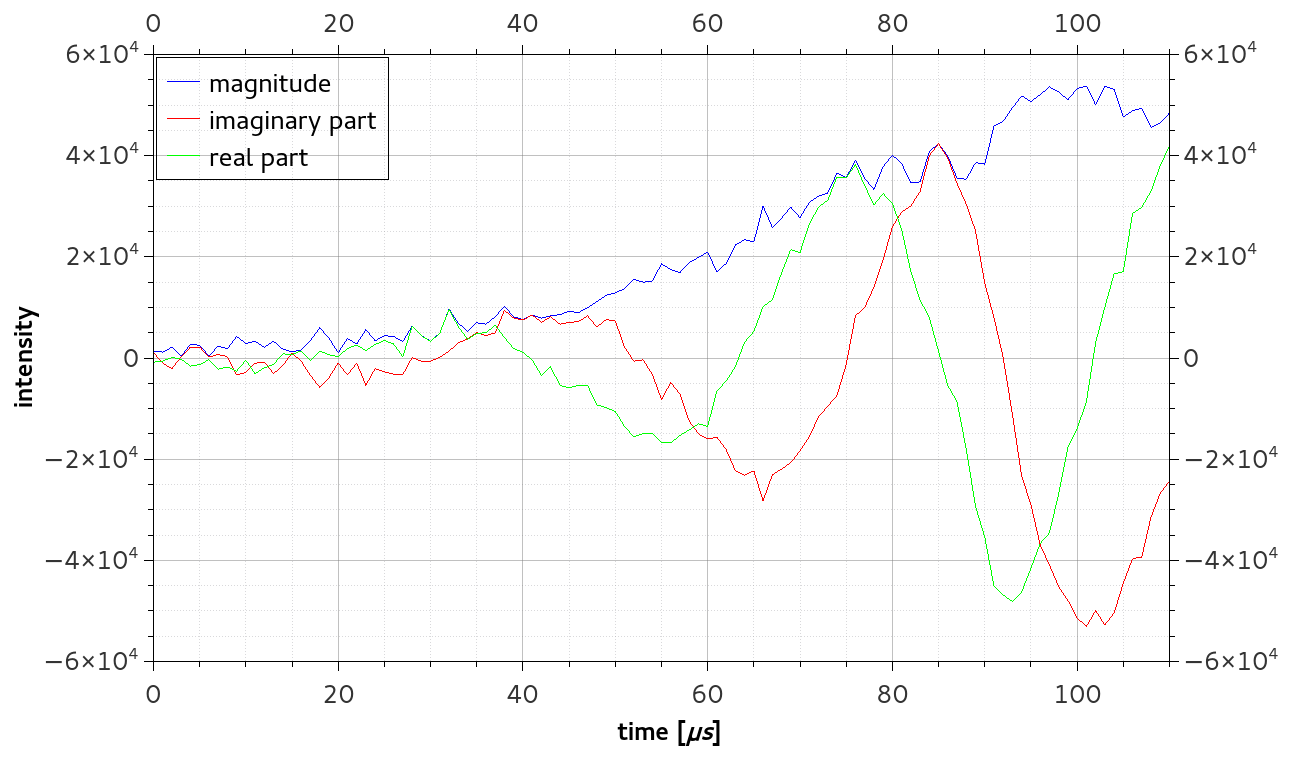
\includegraphics[scale=0.24]{pic/above_resfreq_td.png}}
            \subfigure[intensity below resonance frequency in fourier space\label{abofs}]{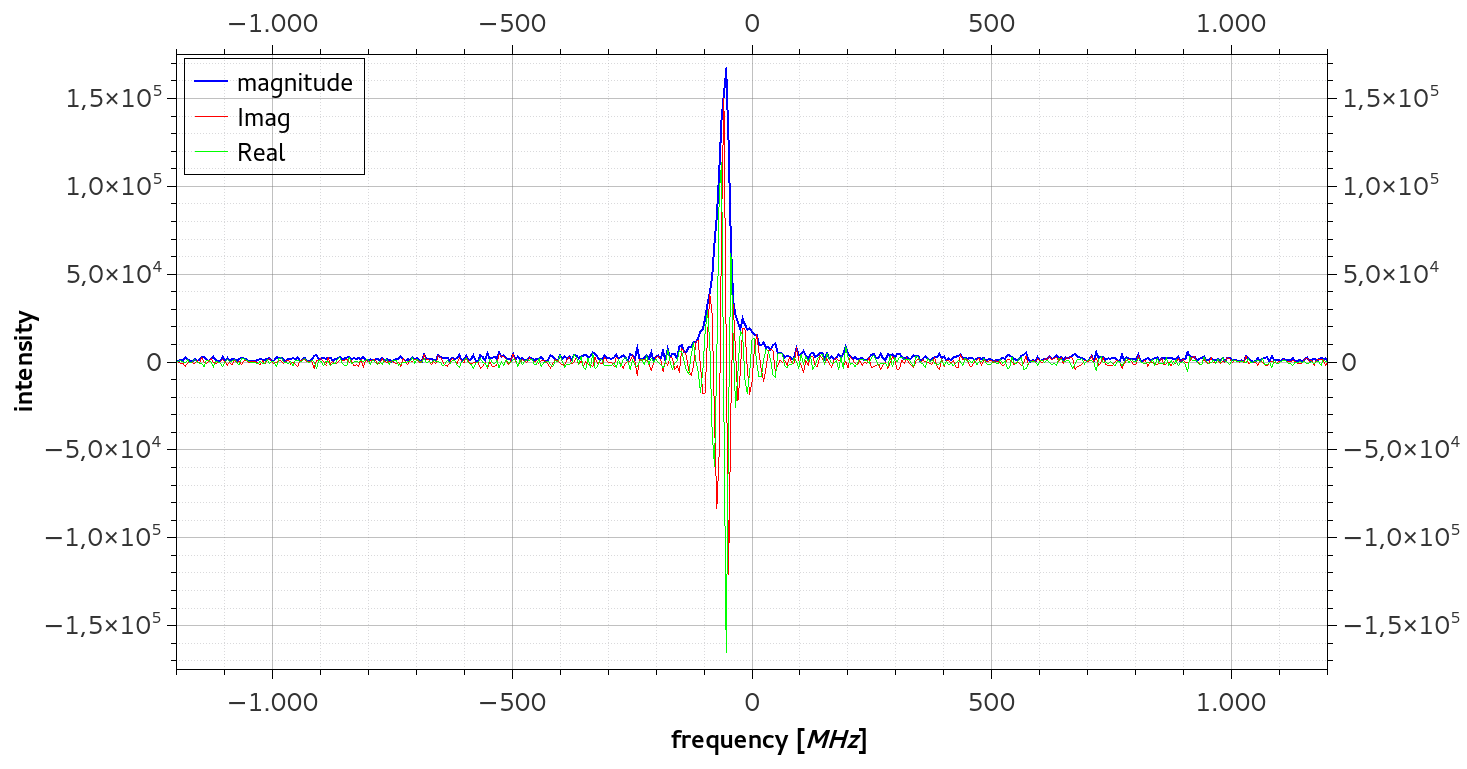
\includegraphics[scale=0.225]{pic/above_resfreq_fs.png}}
            \caption{Different spectra below, at and above the resonance frequency}
         \end{figure}
         
         
    \subsection{Optimization of the pulse sequence by recording a roation angle curve}
    \label{task_3}
    
    \subsection{Finding of $T_1 \text{ and } T_2$}
    \subsubsection{Spin-Lattice relaxation constant}
    \begin{figure}[h]
            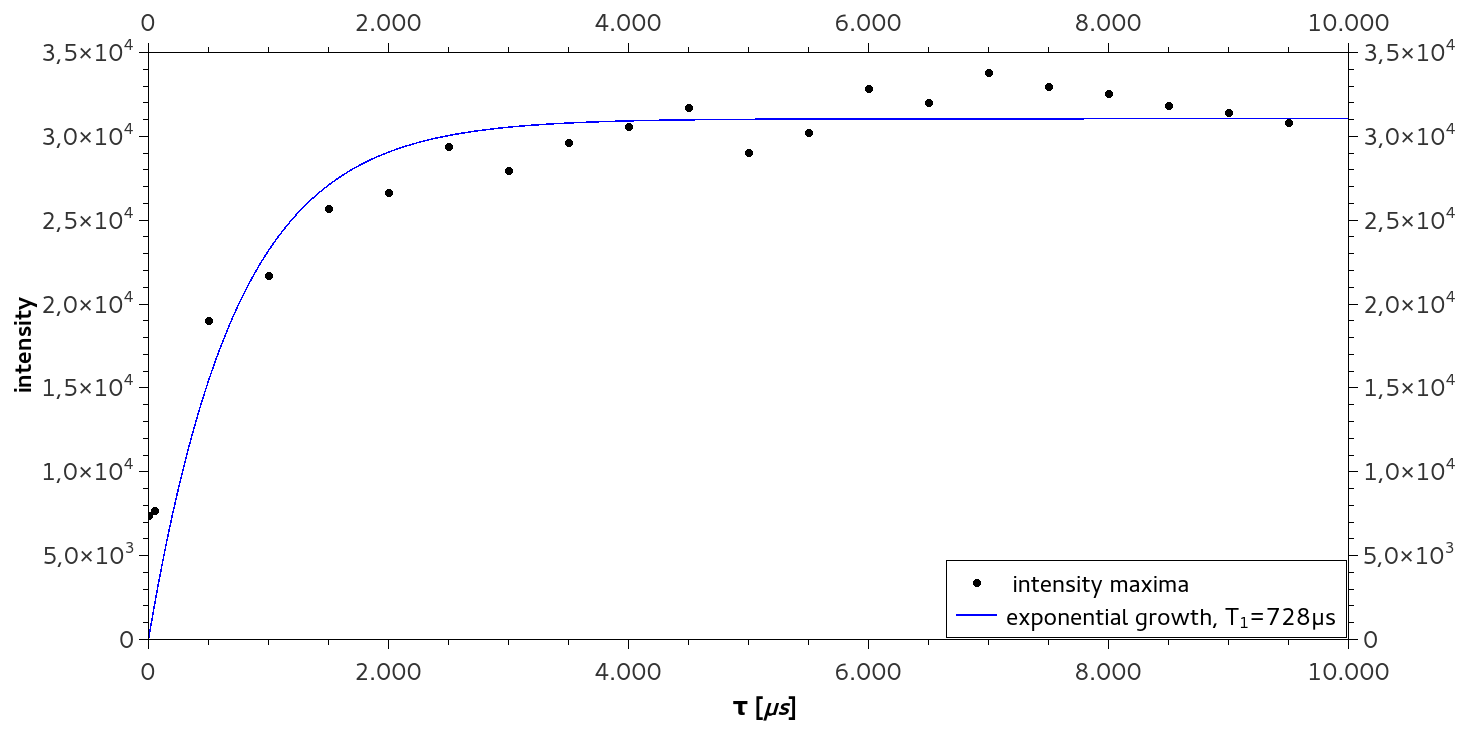
\includegraphics[scale=0.3]{pic/T1.png}
            \captionof{figure}{fit of a spin}
    \end{figure}
    \subsubsection{Spin-Spin relaxation constant}
    \begin{figure}
            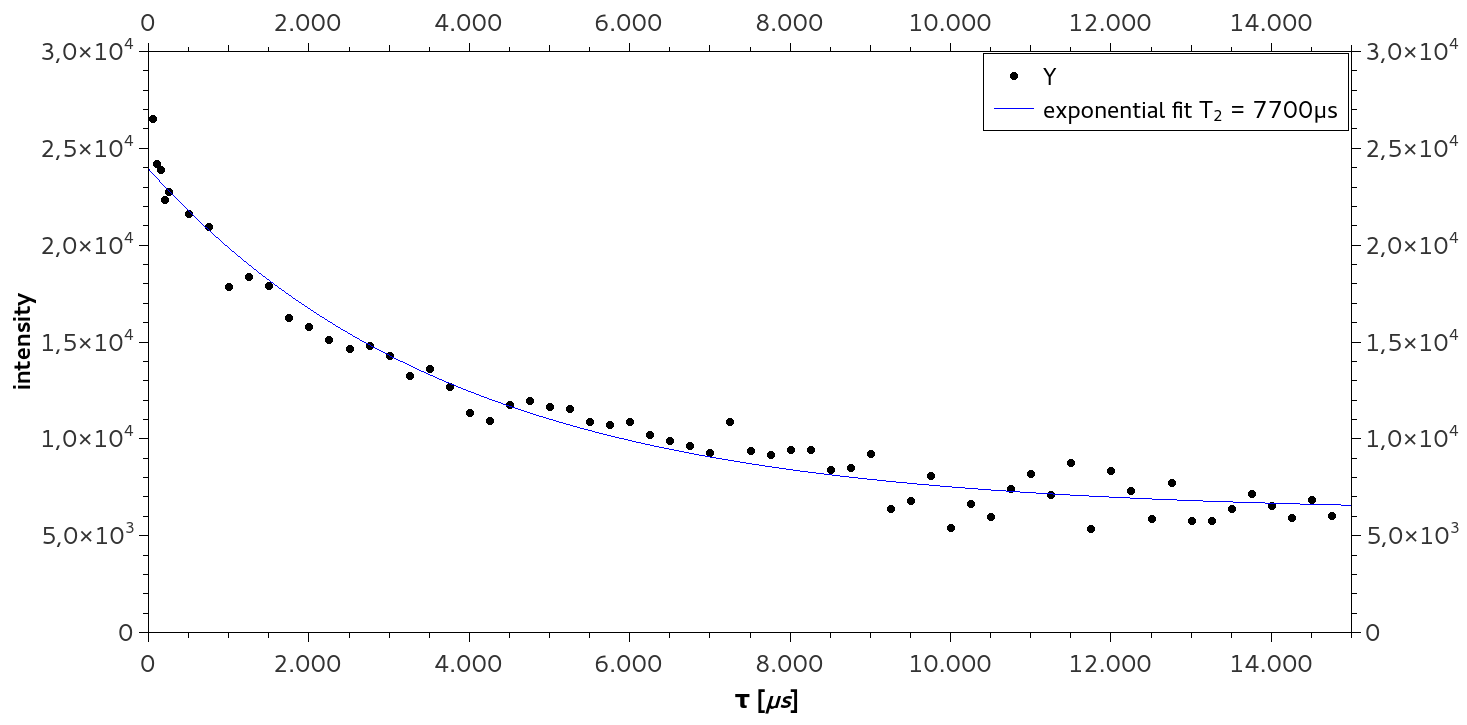
\includegraphics[scale=0.3]{pic/T2.png}
    \end{figure}
    
    \label{task_4}